\documentclass[xcolor=svgnames]{beamer}
\usepackage[utf8]{inputenc}
\usepackage[english]{babel}

\newcommand{\semitransp}[2][35]{\color{fg!#1}#2}
\usepackage{wrapfig}

\usetheme{Proso}

\title[slepemapy.cz]{Adaptabilní výukový systém pro učení faktických znalostí zeměpisu}
\author{Vít Stanislav}
\institute{Fakulta informatiky Masarykovy univerzity}      % Enter your institute name between curly braces
\date{22. 6. 2015}

\begin{document}
% --------------------------- SLIDE --------------------------------------------
\frame[plain]{\titlepage}
% ------------------------------------------------------------------------------
% --------------------------- SLIDE --------------------------------------------
\begin{frame}
	\frametitle{Obsah}
  \begin{itemize}
  \huge \item Systém z pohledu uživatele
%- uzivatelsky pohled: procvičování, mapa znalostí, přehled map
% - počet map / obsah
  \huge \item Systém z pohledu vývojáře
%- architektura
 %- rozdělení práce
 %- použité technologie 
 %- modelovani a predikce
%- časový harmonogram
  \huge \item Související systémy a výzkum
%- použití
%- počet uživatelů / použití / 
%- odkud přicházi? - z googlu
%- překlady en/es/de
%- další systémy
%- výzkum na datech
%- ocenění
  \end{itemize}
\end{frame}
% --------------------------- SLIDE --------------------------------------------
\begin{frame}
	\frametitle{Procvičování států}
   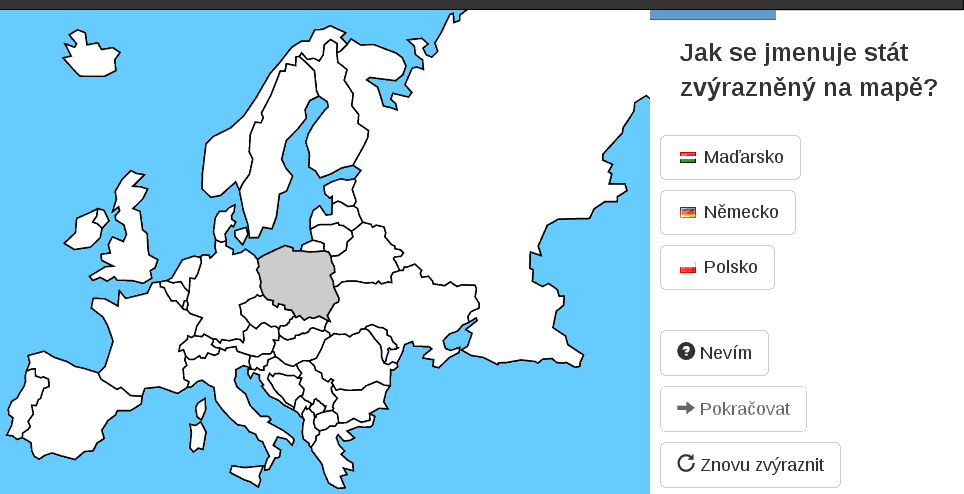
\includegraphics[width=\textwidth]{img/practice-example-cs.png}
\end{frame}
% ------------------------------------------------------------------------------
% --------------------------- SLIDE --------------------------------------------
\begin{frame}
	\frametitle{Mapa znalostí}
   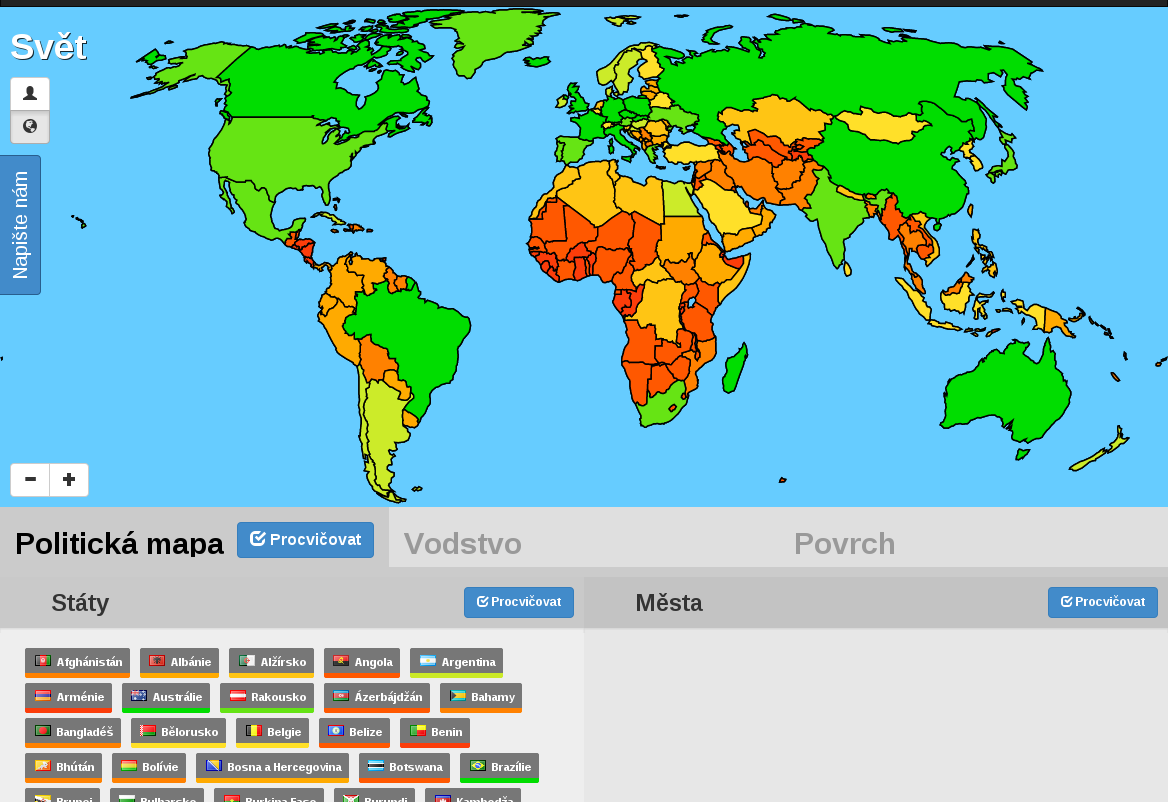
\includegraphics[width=\textwidth]{img/knowledge-map-world.png}
\end{frame}
% ------------------------------------------------------------------------------
% --------------------------- SLIDE --------------------------------------------
\begin{frame}
	\frametitle{Přehled map}
   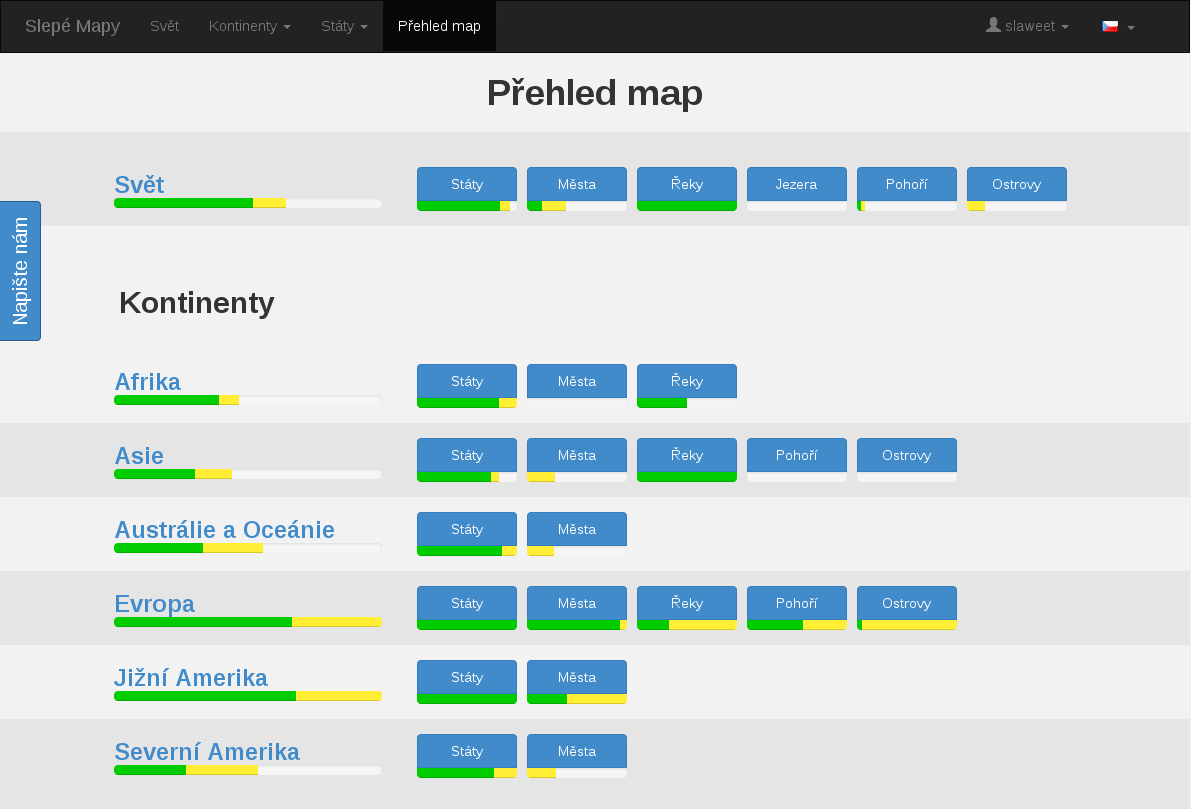
\includegraphics[width=\textwidth]{img/overview.png}
\end{frame}
% ------------------------------------------------------------------------------
% --------------------------- SLIDE --------------------------------------------
\begin{frame}
	\frametitle{Obsah}
  \begin{itemize}
  \semitransp[20]{
  \huge \item Systém z pohledu uživatele
}
  \semitransp[100]{ 
  \huge \item Systém z pohledu vývojáře
  }
  \semitransp[20]{
  \huge \item Související systémy a výzkum
}
  \end{itemize}
\end{frame}
% --------------------------- SLIDE --------------------------------------------
% --------------------------- SLIDE --------------------------------------------
\begin{frame}
	\frametitle{Architektura systému}
   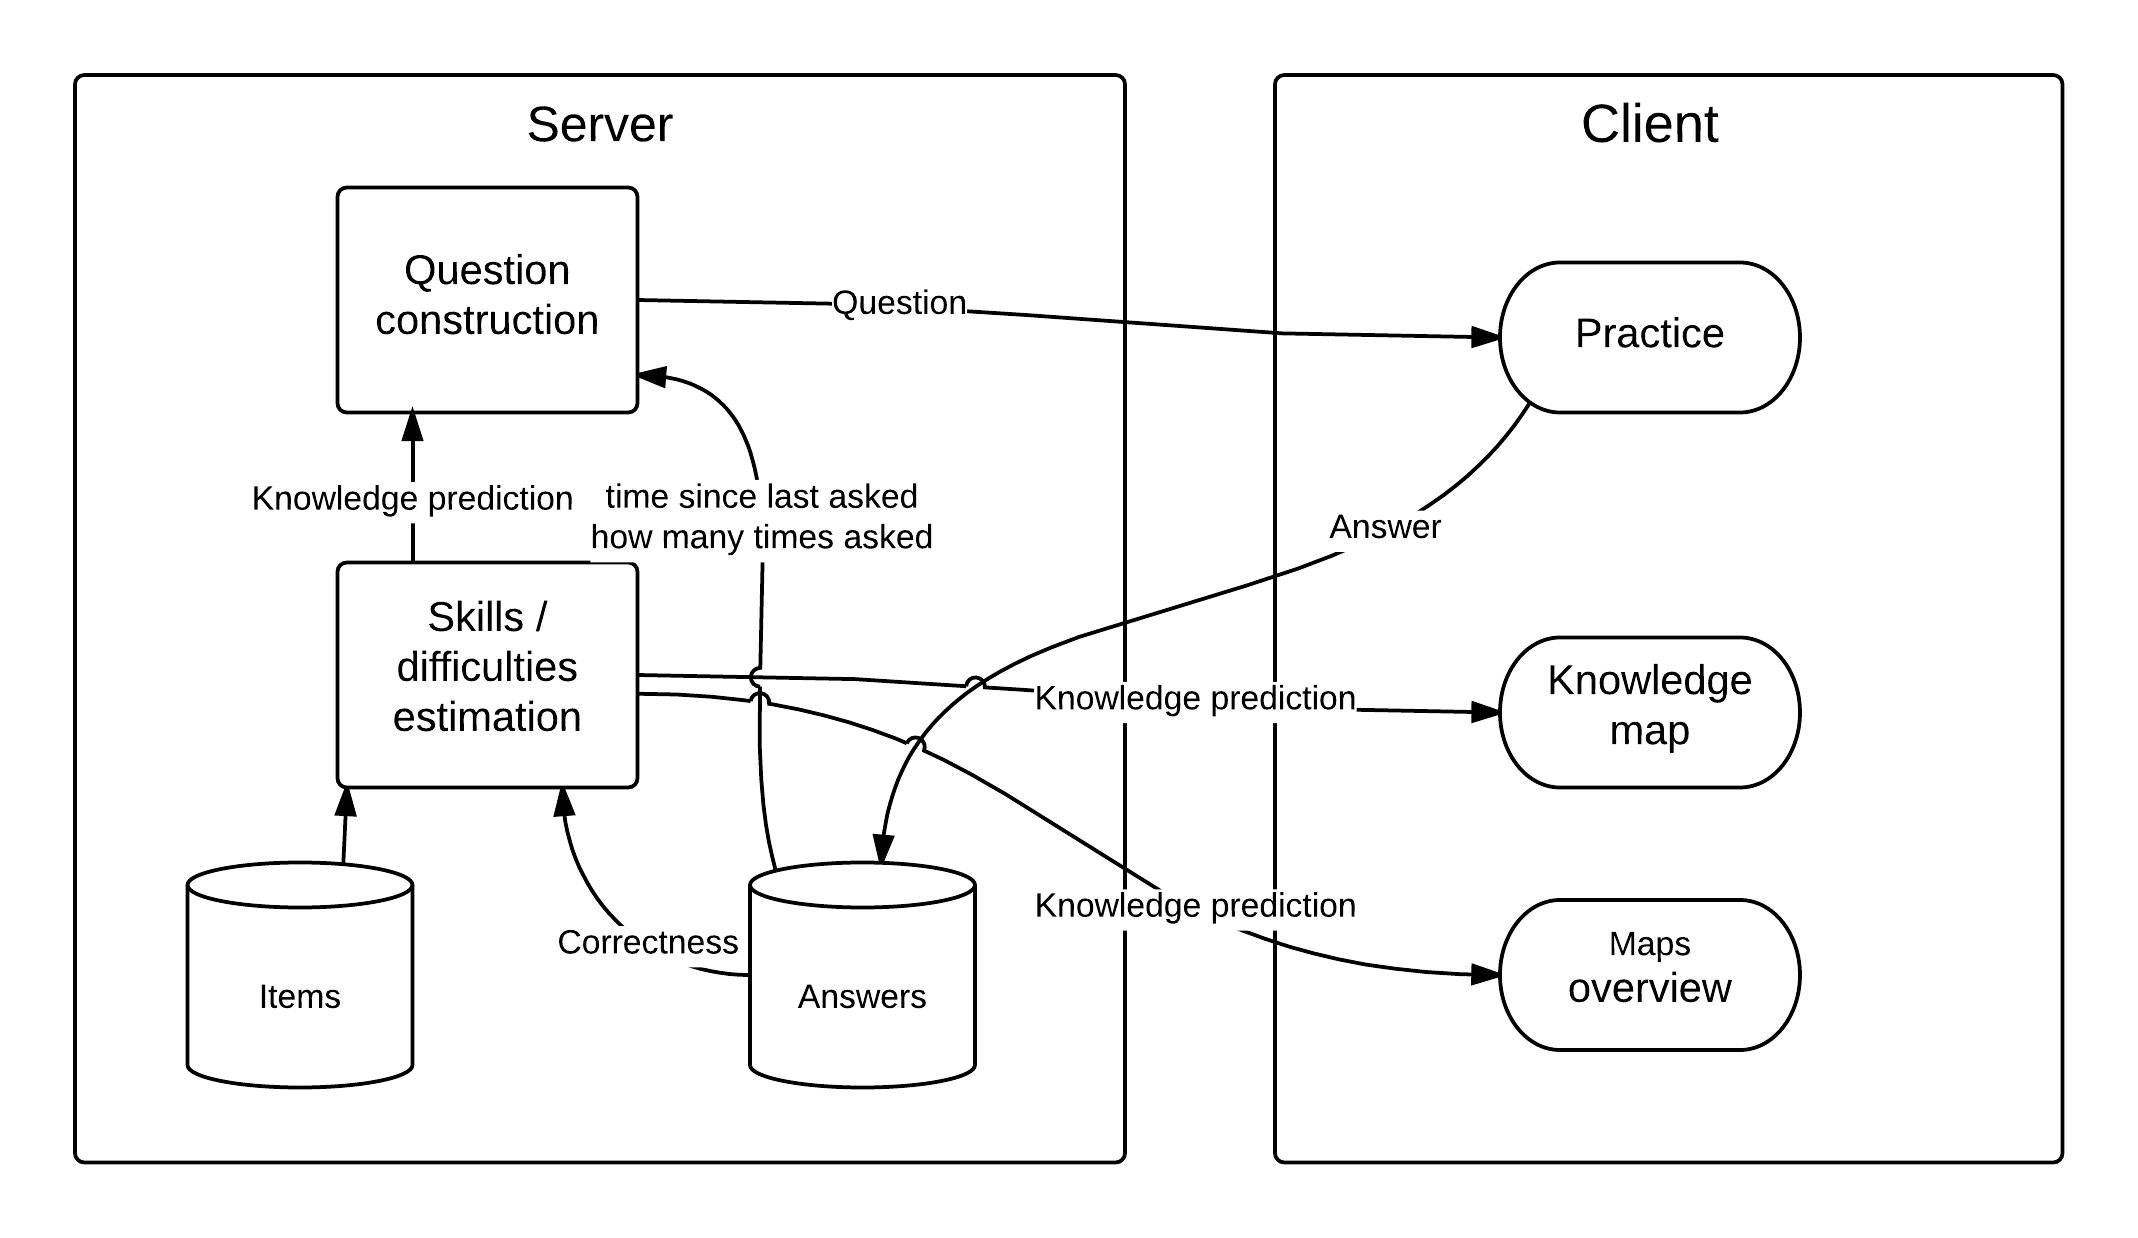
\includegraphics[width=\textwidth]{img/architecture.png}
\end{frame}
% ------------------------------------------------------------------------------
% --------------------------- SLIDE --------------------------------------------
\begin{frame}
	\frametitle{Výběr vhodných otázek}
  \begin{columns}
   \begin{column}{.49\textwidth}
      Odhad parametrů z odpovědí uživatelů 
      \begin{itemize}
        \item obtížnost státu
        \item celková znalost uživatele
        \item znalost daného státu 
      \end{itemize}
      Výběr otázky 
      \begin{itemize}
        \item přiměřená obtížnost 
        \item otevřená nebo s 2~-~6 možnostmi
        \item výběr možností
      \end{itemize}
    \end{column}
    \begin{column}{.49\textwidth}
       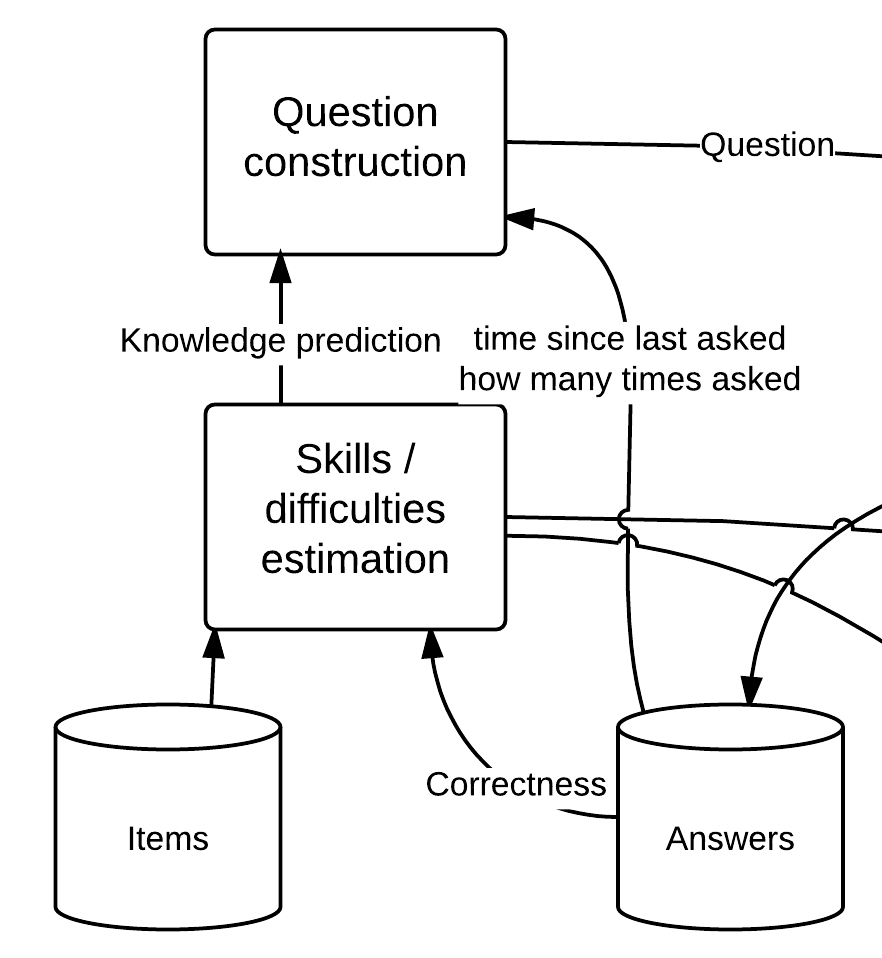
\includegraphics[width=\textwidth]{img/architecture-server.png}
    \end{column}
  \end{columns}
\end{frame}
% ------------------------------------------------------------------------------
% --------------------------- SLIDE --------------------------------------------
\begin{frame}
	\frametitle{Projekt v čase}
  \begin{itemize}
    \item \textbf{Vývoj beta verze} (červen -- listopad 2013
    \begin{itemize}
      \item procvičování států světa
    \end{itemize}
    \item \textbf{Studentský projekt na FI} (prosinec 2013 -- květen 2014)
    \begin{itemize}
      \item podpora pro města, řeky, jezera, apod.
      \item přehled map
      \item SEO
    \end{itemize}
    \item \textbf{Projekt z CTT} (srpen -- prosinec 2014)
    \begin{itemize}
      \item internacionalizace a anglická lokalizace
      \item osobní cíle
      \item anketa obtížnosti otázek
    \end{itemize}
  \end{itemize}
\end{frame}
% ------------------------------------------------------------------------------
% --------------------------- SLIDE --------------------------------------------
\begin{frame}
	\frametitle{Provoz aplikace}
  \begin{itemize}
    \item 200 000 návštěv a 10 milionů odpovědí celkem
    \item 20 000 návštěv a 1 milion odpovědí za poslední měsíc
  \end{itemize}
   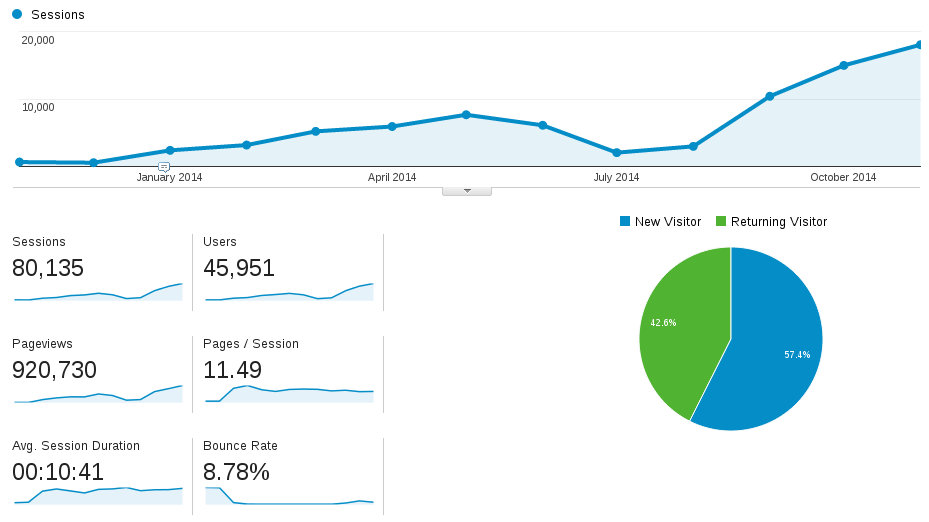
\includegraphics[width=\textwidth]{img/audience.png}
\end{frame}
% ------------------------------------------------------------------------------
% --------------------------- SLIDE --------------------------------------------
\begin{frame}
	\frametitle{Návštěvnost během dne}
	 
   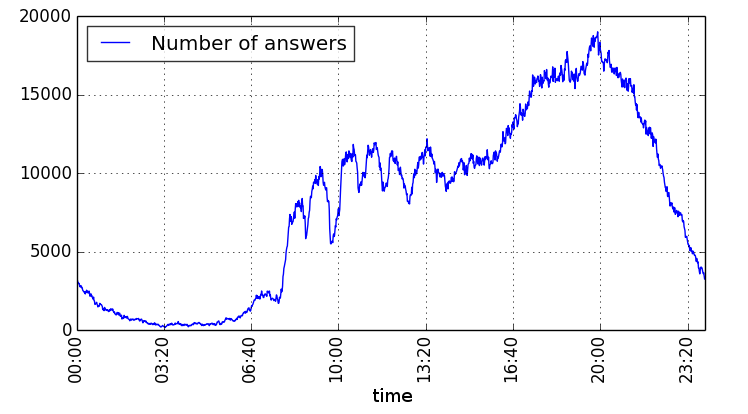
\includegraphics[width=\textwidth]{img/answers_in_day_by_minute_absolute.png}
\end{frame}
% ------------------------------------------------------------------------------
% --------------------------- SLIDE --------------------------------------------
\begin{frame}
	\frametitle{Obsah}
  \begin{itemize}
  \semitransp[20]{
  \huge \item Systém z pohledu uživatele
  \huge \item Systém z pohledu vývojáře
}
  \semitransp[100]{ 
  \huge \item Související systémy a výzkum
  }
  \end{itemize}
\end{frame}
% --------------------------- SLIDE --------------------------------------------
% --------------------------- SLIDE --------------------------------------------
\begin{frame}
	\frametitle{autoskolachytre.cz}
	 
   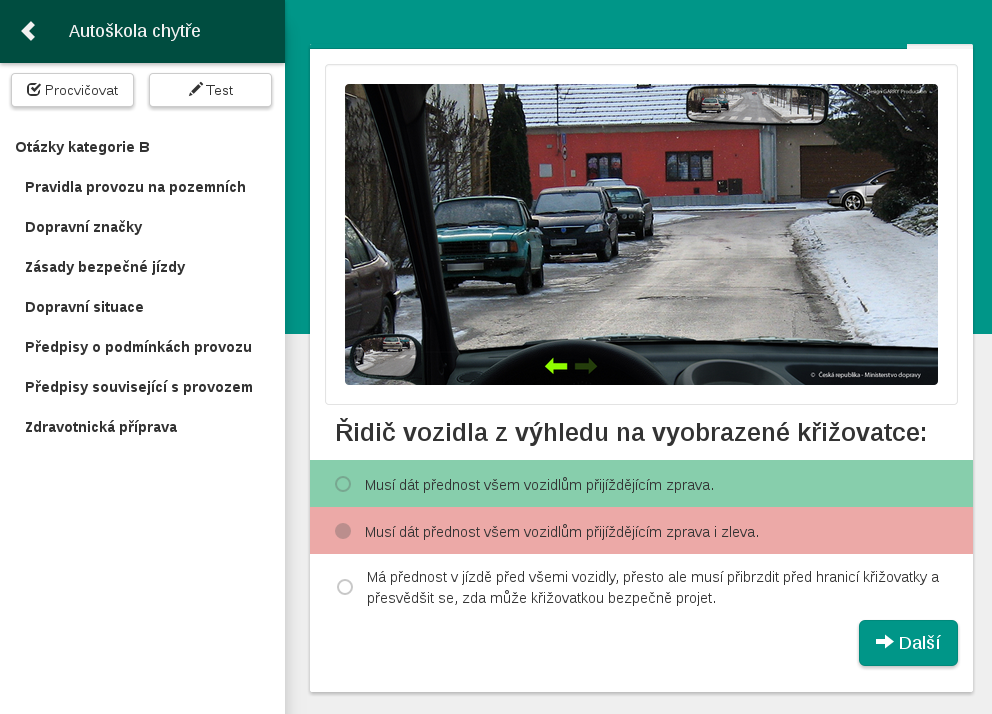
\includegraphics[width=\textwidth]{img/autoskola.png}
\end{frame}
% ------------------------------------------------------------------------------
% --------------------------- SLIDE --------------------------------------------
\begin{frame}
	\frametitle{anatom.cz}
	 
   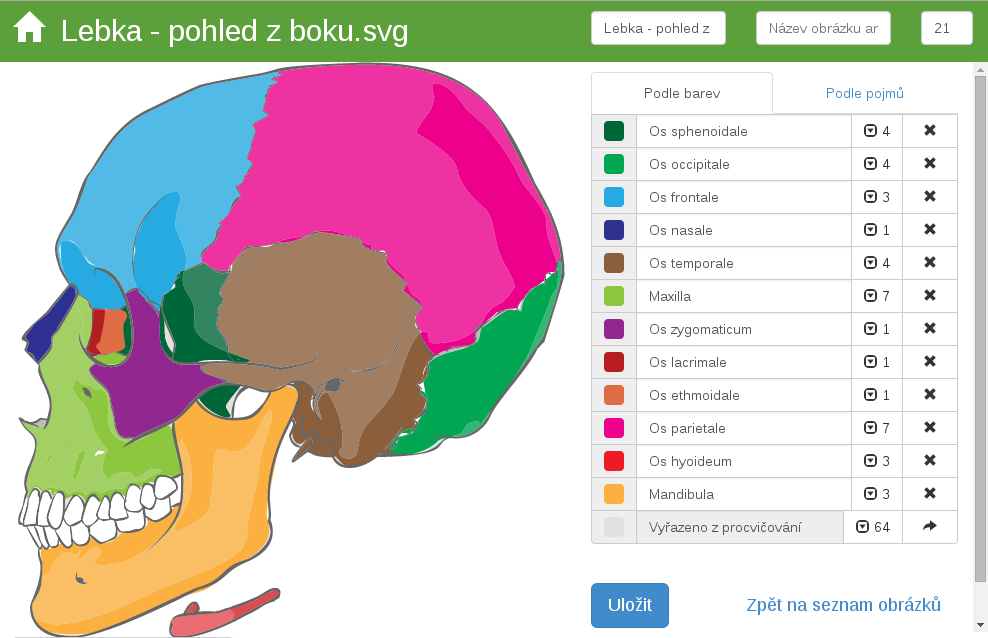
\includegraphics[width=\textwidth]{img/anatomie.png}
\end{frame}
% ------------------------------------------------------------------------------
% --------------------------- SLIDE --------------------------------------------
\begin{frame}
	\frametitle{Výzkum na posbíraných datech}

  \begin{itemize}
   \item \textbf{Adaptabilní procvičování}

  \begin{itemize}
   \item J. Papoušek, R. Pelánek, V. Stanislav. Adaptive Practice of Facts in Domains with Varied Prior Knowledge. Educational Data Mining (EDM), 2014.
   \item J. Papoušek, R. Pelánek. Impact of Adaptive Educational System Behaviour on Student Motivation. Artificial Intelligence in Education (AIED), 2015.
   \item J. Papoušek, R. Pelánek, J. Řihák, V. Stanislav. An Analysis of Response Times in Adaptive Practice of Geography Facts. Educational Data Mining (EDM), 2015.
  \end{itemize}

   \item \textbf{Modelování studentů }

  \begin{itemize}
   \item R. Pelánek. Metrics for Evaluation of Student Models. Journal of Educational Data Mining, 2015.
   \item J. Nižnan, R. Pelánek, J. Řihák. Student Models for Prior Knowledge Estimation. Educational Data Mining (EDM), 2015.
  \end{itemize}
  \end{itemize}

\end{frame}
% ------------------------------------------------------------------------------
% --------------------------- SLIDE --------------------------------------------
\begin{frame}
	\frametitle{Další závěrečné práce}
  \begin{itemize}
  \item Dionýz Lazar - Analýza dat ze systému pro výuku zeměpisu (bakalářská práce)
  \item Jan Kučera - Adaptabilní webový systém pro výuku anatomie, slepaanatomie.cz (diplomová práce)
  \end{itemize}
\end{frame}
% ------------------------------------------------------------------------------
% --------------------------- SLIDE --------------------------------------------
\begin{frame}
  \frametitle{~}
\begin{center} 
\huge  Děkuji za pozornost.
\end{center}
\end{frame}
% ------------------------------------------------------------------------------
\end{document}
